%!TEX root = ../vernier.tex
\chapter{Metric Collection} \label{sec:metrics}

Software Quality Metrics are measurements that relate to properties of a piece of software or its specifications. They can generate useful insight in various levels of granularity (e.g. project level, package level, class level, method level) and can lead to a better understanding of the code base. These insights might influence several decisions, ranging from where to place refactoring and performance optimization effort to budget planning, optimal personnel task assignments, and cost estimation.

\begin{figure}[H]
	\centering
	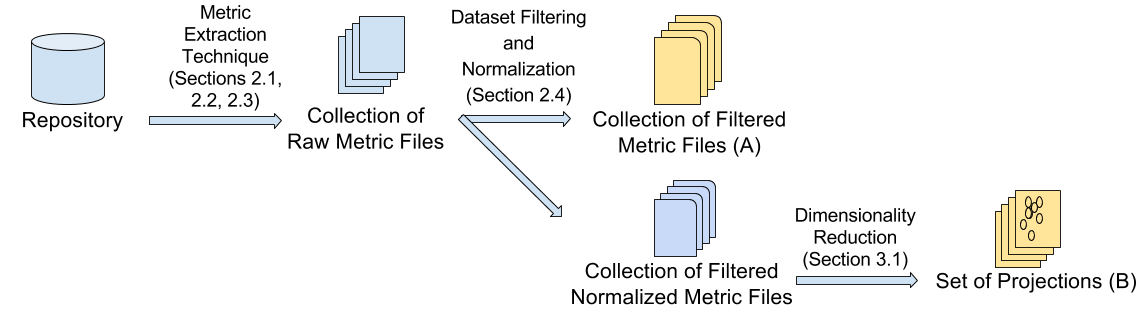
\includegraphics[width=\textwidth]{figures/pipeline.png}
	\caption{Data extraction pipeline}
	\label{fig:data_pipeline}
\end{figure}

Figure \ref{fig:data_pipeline} illustrates the pipeline that takes a software repository and outputs the two datasets (A and B) that are used in our visualization tool.

The first step to collecting data from repositories is choosing what Version Control Systems to use. There are many options such as Subversion, Perforce, Mercurial, Bazaar, CVS, and Git. To choose one over the others, aspects such as popularity for Open Source projects, efficiency in the use of resources, performance, and simplicity to "walk" between revisions are taken into consideration. More details on the discussion are presented on Section \ref{sec:git}

The choice of Metric Extraction tool is discussed in Section \ref{sec:understand}.

The method developed to take revision files and generate a collection of raw metric tables scalably is featured on Section \ref{sec:extraction}.

The need for filtering and normalization of the acquired datasets is explained on Section \ref{sec:filtering}.

\section{Version Control System} \label{sec:git}

In order to estimate VCS popularity, we will use Google Trends data collected from January 2004 to November 2016 on the most used systems according to the 2015 Stack Overflow Developers Survey \cite{ref:stackoverflow}. Google Trends allows comparison between the number of Google searches related to a particular system relative to the total search volume. A world map also points out which is the most popular system in each country.

\begin{figure}[H]
	\centering
	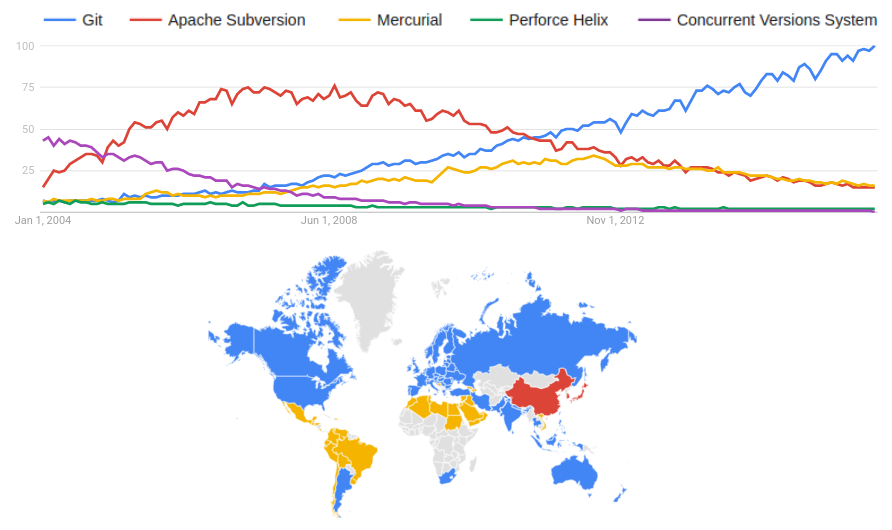
\includegraphics[width=\textwidth]{figures/vcs_pop.png}
	\caption{The variable in the graph represents the global search interest relative to the highest point on the chart through time.}
	\label{fig:vcs_pop}
\end{figure}

Based on this data, we can confirm that Git is currently the most popular VCS and that it's popularity is steadily increasing.

According to GitHub co-founder Scott Chacon on the book Pro Git \cite{ref:progit}, the major difference between Git and any other VCS is the way Git "thinks" about its data. Conceptually, most other systems (e.g. SVN, Mercurial and CVS) store information as a list of file-based changes, meaning that in a source file with a hundred lines of code, if three new lines are added, only these three lines with their meta data are going to be stored in the new revision. Git, instead, stores its data as a series of snapshots of the file system, which mean that the hundred and three lines of code are redundantly (even though compressed) saved into the repository when the changes are committed.

Despite that, according to \citet{ref:gitwiki}, Git is much faster than Subversion since all operations (except for push and fetch) are local and there is no network latency. Git's repositories are also much smaller than Subversions (for the Mozilla project, 30x smaller) and Git repository clones act as full repository backups.

One of the reasons for the smaller repository size is that an SVN working directory always contains two copies of each file: one for the user to actually work with and another hidden in the \textit{.svn/} folder to aid operations such as status, diff and commit. In contrast a Git working directory requires only one small index file that stores about 100 bytes of data per tracked file. On projects with a large number of files this can be a substantial difference in the disk space required per working copy.

Every time a commit is made in Git, the differences are not recorded, instead, it saves all modified files integrally and inserts their references to the commit tree. To be efficient, if files have not changed, they are not redundantly stored in disk, but a link to the previous identical file it has already stored is created. Therefore, Git thinks about its data dynamics as a stream of snapshots. The organization of a repository tree is depicted on Figure \ref{fig:git_architecture}.

\begin{figure}[h]
	\centering
	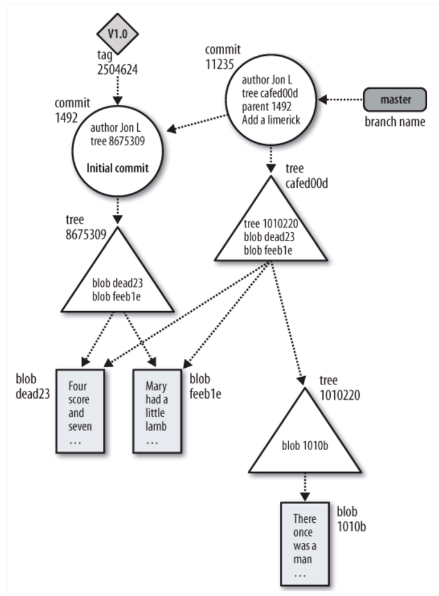
\includegraphics[width=0.7\textwidth]{figures/git_architecture.png}
	\caption{Git tree organization}
	\legend{Source: \url{https://www.hackerearth.com/}}
	\label{fig:git_architecture}
\end{figure}

Subversion has the advantage of having a simpler way to navigate between revisions as it uses sequential revision identifiers (1,2,3,..), instead of Git's unpredictable SHA-1 hashes.

Considering the popularity factor, full local repository backups with integral files, better performance and use of resources, we deemed Git as being a more suitable system for our context. Additionally, the well documented and maintained library \textit{libgit2} for C/C++ was fundamental for the choice of VCS.

\section{Software Quality Metrics Extraction Tools} \label{sec:understand}

Our requirements for the Software Quality Metrics Extractor Tool regarded the quality and relevance of the metrics, strictness of input acceptance (e.g. how it dealt with unbuildable code and missing references), project activity, overall performance and ease of set-up and integration. It is important for the understanding of the project dynamics to extract both intra-file metrics, i.e. those which can be computed simply by looking at a single file in isolation (e.g. number of lines of code, average method complexity, average class cohesion) and inter-file metrics, which are metrics that look at the relations between entities in different files (e.g. depth of a class hierarchy, average function-call-path length, metrics on the number of uses of a given symbol). The latter are significantly more complex to compute.

Eight tools were tested in the metric extractor tools analysis phase of the study, out of which, four - CCCC, SourceMeter, iPlasma and CppCheck - were swiftly discarded due to design or performance misalignment with our goals. The remaining four tools - SonarQube, Analizo, CodePro Analytix and SciTools Understand - were subjected to a series of tests that would grade the suitability of each for our purposes.

SonarQube is a very professional tool dedicated to continuous analysis and measurement of source code. It has complicated initial set-up and proved to be hard to integrate in our software. The quality of its outputted metrics wasn't on par with the other three tools and it’s performance wasn’t satisfactory either.
Analizo, differently from the other three tools, is an academic project. It is easy to use and outputs a good amount of relevant metrics. Unfortunately, for complicated projects with many external or missing references, it struggled, taking over 30 minutes to analyze medium size repositories, rendering it unsuitable for our study.

CodePro Analytix and SciTools Understand fit all our requirements. Both are easy to use and integrate, flexible regarding the repositories they take as input, customizable in the parameterization of the metrics, fast, well-documented professional grade tools. Both output a good set of inter and intra-file metrics in various levels of granularity and in easy to work formats (xml and csv). We chose to work with Understand over Analytix in reason of the performance advantage one has over the other and the number of class level metrics they output (43 for Understand against Analytix’s 17). The full metric reference document provided by SciTool Understand is available at \cite{ref:und}.

Table \ref{tab:und_ana_times} shows the performance comparison between the two tools for nine Open Source projects.
% TODO: perhaps do a nice visualization of the table
\begin{table}[ht]
	\caption{Understand and Analytix analysis time for a single revision}
	\centering
	\label{tab:und_ana_times}
	\begin{tabular}{c|c|c}
		\hline
		\textit{Project (KLOC)} & \textit{Analytix Time(s)} & \textit{Understand Time(s)} \\
		\hline
		\hline
		JMeter (118)            & 23                        & 30                          \\
		Checkstyle (95)         & 32                        & 32                          \\
		Gitblit (77)            & 31                        & 20                          \\
		JUnit (26)              & 17                        & 10                          \\
		JavaGame (3)            & 10                        & 4                           \\
		Netty (194)             & 70                        & 66                          \\
		Guava (243)             & 120                       & 168                         \\
		Zxing (42)              & 20                        & 11                          \\
		MPAndroidChart (20)     & 14                        & 8                           \\
		\hline
	\end{tabular}
\end{table}


Table \ref{tab:comp} shows a score from 0 to 5 related to requirements measured on each tool. In order to fit all data in one table, we labeled the requirements in the following fashion:

\begin{table}[ht]
	%\caption{Uma tabela de Exemplo}
	% OBS: não use \begin{center}, pois este aumenta o espaçamento entre a caption/legend e a tabela
	% Para figuras, a aparência é melhor com o espaçamento extra
	\centering
	\begin{tabular}{c|c}
		\hline
		\textit{Requirement}          & \textit{Label} \\
		\hline
		\hline
		Well maintained               & A              \\
		Ease to set up                & B              \\
		Easy to integrate             & C              \\
		Tolerance of input acceptance & D              \\
		Metric Quality                & E              \\
		Performance                   & F              \\
		\hline
	\end{tabular}
	%\legend{Fonte: Os Autores}
	\label{tbl:ex1}
\end{table}

\begin{table}[H]
	\centering
	\caption{Tool Comparison: Some cells have dashes instead of values because the tool was considerate unsuitable before the attribute was measured.}
	\label{tab:comp}
	\begin{tabular}{c|c|c|c|c|c|c}
		\hline
		\textit{Tool} & \textit{A} & \textit{B} & \textit{C} & \textit{D} & \textit{E} & \textit{F} \\
		\hline
    \hline
		CCCC          & 0          & 0          & -          & 0          & -          & -          \\
		Source Meter  & 3          & 0          & -          & -          & -          & 1          \\
		iPlasma       & -          & 4          & 0          & -          & 1          & 2          \\
		CppCheck      & -          & -          & -          & -          & 0          & -          \\
		SonarQube     & 5          & 1          & 3          & 4          & 2          & 2          \\
		Analizo       & 3          & 3          & 3          & 2          & 5          & 2          \\
		Analytix      & 5          & 4          & 5          & 5          & 4          & 4          \\
		Understand    & 5          & 4          & 5          & 5          & 5          & 5          \\
    \hline
  \end{tabular}
\end{table}

\section{Metric Extraction} \label{sec:extraction}
Once we had settled on Git and Scitools Understand as VCS and metric collector, we built a tool that takes as argument a repository URL (e.g. \url{https://github.com/google/ExoPlayer.git}) or a path to an already checked-out on disk repository and outputs a collection of files that represent the metric values for a set of revisions. The number $n$ of revisions to be extracted from the repository is also given as an argument along with an optional $T_{start}$ -- $T_{end}$ interval. The JMeter project, for example, has currently 12,647 commits. If we input 100 as the number of revisions, the first to be extracted will be the last committed revision, after that, we walk 126 steps back on the commit tree and check-out the next one. The process continues consecutively for the remaining revisions.

We thought of two approaches to perform metric extraction. The first would be to create $n$ directories and for each of them, check-out all source files from the $i$th revision. This is the easiest method but it is slow and space inefficient, as files from previous commits that have not undergone changes must be decompressed and written to disk unnecessarily.

The second approach was the one we chose to work with. First, check-out every Java source file from the last revision to a single "dump" directory, disregarding the original directory structure. Considering Git keeps all it's past files compressed in the .git folder, this process is very fast and requires no online access to the repository --- this is crucial, considering the operation is repeated several times.

With all files checked-out in the dump directory, all alphanumeric SHA-1 file and directory keys (which work as identifiers) listed in this commit are added to a Trie data structure. Understand then runs it's metric calculations and outputs an appropriately identified file to the \textit{metric} directory.

When the metric calculation is complete, it takes the next selected commit and, comparing it's file/directory keys to the current state on the Trie tree, checks which files or groups of files are already loaded into disk. It also checks which of the files that are currently checked into disk are not present in the next revision and deletes them. The Trie tree is then updated for the current revision. The quality metrics are then extracted and this step is repeated for the remaining $n-1$ revisions.

The \textit{metric} directory for the JMeter project with 20 analyzed revisions looks like Figure \ref{fig:jmeter_folder} where each file is CSV formatted collection of 43 attributes.

\begin{figure}[H]
	\centering
	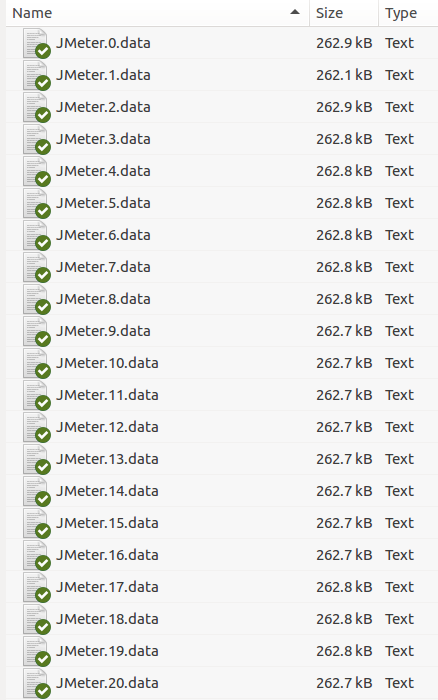
\includegraphics[width=0.6\textwidth]{figures/metric_dir.png}
	\caption{Metric output file set}
	\label{fig:jmeter_folder}
\end{figure}

More details and source code can be found at \url{https://github.com/EduardoVernier/metric-extractor}. The tool was implemented in C++ with the Qt framework.

\section{Dataset Filtering and Normalization} \label{sec:filtering}
Before the datasets are ready for the visualization two last steps are necessary. The first concerns the unsuitability of current dimensionality reduction technique to deal with dynamic datasets, i.e. collections where members are created or deleted between consecutive time moments. What this implies is that all classes that we are analyzing must be present from the first selected commit up until the last one, which means that a considerable percentage of the project's classes must be filtered from the dataset. As far as we know, no multidimensional projection technique fits this requirement.

The second step is normalization. This is necessary because some metric range from 0 to 1 (e.g comments ratio) and others don't have a specific delimited range (e.g lines of code), therefore the dimensionality reduction technique will associated different weights to different metric value changes (which is not ideal). To perform the data normalization, we must first extract the average value and standard deviation of each attribute. Then for each sample, we subtract the corresponding average and divide the result by the standard deviation. What this guarantees is that the average for each feature is zero and the standard deviation through time is one, allowing unbiased projection calculations.
